\documentclass[11pt, notheorems]{beamer}

\usetheme{Warsaw}
\usecolortheme{seahorse}
\setbeamertemplate{caption}[numbered] % Для включения нумерации рисунков

\usepackage[T1,T2A]{fontenc}
\usepackage[utf8]{inputenc}
\usepackage[english,russian]{babel}
\usepackage{amsthm, amsmath}
\usepackage[
	backend=biber,
	citestyle=gost-footnote-min,
	bibstyle=gost-footnote,
	language=auto,
	autolang=other,
	sorting=none
]{biblatex}

\graphicspath{ {./img/} }
\addbibresource{refs/refs.bib}

\title{Классы унаров, близкие к плоским}
\author{Пряничников А. М.}
% \institute{Overleaf}
\date{2025}

\newtheorem{definition}{Определение}
\newtheorem{theorem}{Теорема}
\newtheorem{corollary}{Следствие}

\begin{document}

\frame{\titlepage}

\begin{frame}
	\frametitle{Полигон}

	\begin{definition}
		Правым \textit{полигоном} над полугруппой $S$ называется множество $X$ с отображением $ X \times S \rightarrow X $, $(x, s) \mapsto xs $ таким, что для любых $x \in X$, $s, t \in S$ выполняется равенство $ x (st) = (xs)t $.
	\end{definition}

	\begin{figure}
		\center
		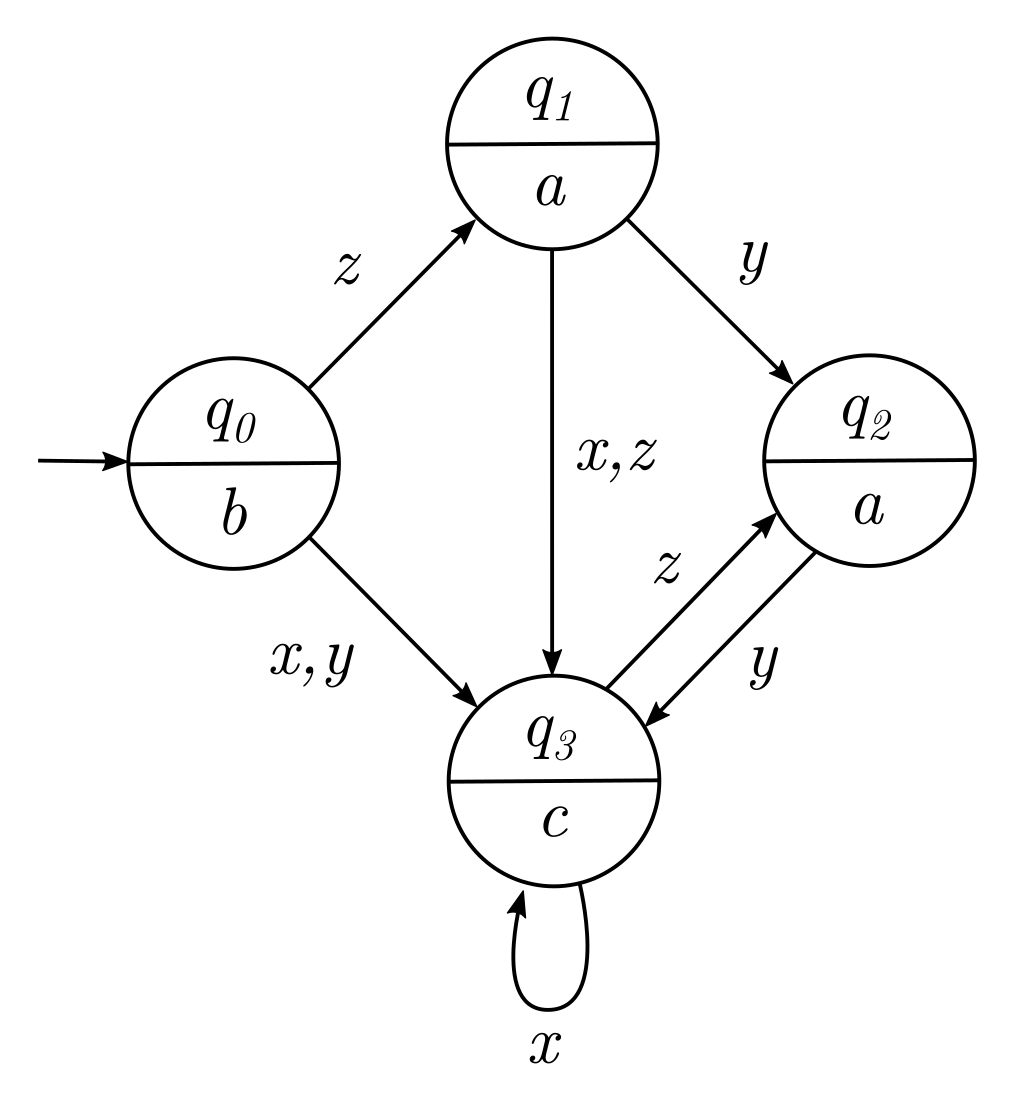
\includegraphics[width=0.3\textwidth]{MooreMachine}
	\end{figure}

	\textit{Копроизведением} $\coprod_{i \in I} X_i$ полигонов $X_i$ над одной полугруппой называется их дизъюнктное объединение.
\end{frame}

\begin{frame}
	\frametitle{Тензорное произведение полигонов}

	Пусть $X_S$ и ${}_{S}Y$ -- соответственно правый и левый полигоны над полугруппой $S$.

	\begin{definition}
		\textit{Тензорное произведение} $X_S \otimes {}_{S}Y$ (или просто $X \otimes Y$) -- это фактор-множество $(X \times Y) / \rho$, где $\rho$ -- наименьшее отношение эквивалентности, содержащее все пары вида $((xs, y),(x, sy))$ для $x \in X$, $y \in Y$, $s \in S$.
	\end{definition}

	Класс, в котором лежит пара $(x, y)$, обозначается $x \otimes y$.
	Из определения следует, что для любых $x \in X$, $y \in Y$, $s \in S$ выполняется равенство $ xs \otimes y = x \otimes sy$.

\end{frame}

\begin{frame}
	\frametitle{Плоскостность}

	\begin{definition}
		Морфизм $f: A \rightarrow B$ в категории $\mathcal{C}$ называется \textit{мономорфизмом}, если на него можно сократить слева, то есть выполняется импликация:
		если $f \circ k = f \circ h$, то $k = h$ для любых $k, h \in \mathrm{Mor} \ (C, A)$.
	\end{definition}

	\begin{definition}
		Полигон $X$ называется плоским, если функтор $X \otimes - $ сохраняет мономорфизмы.
	\end{definition}

	$$ F_{X_S} ({}_{S}Y) = X_S \otimes {}_{S}Y $$

	$$ F_{X_S}: S-\textbf{Act} \rightarrow \textbf{Set}$$
\end{frame}

\begin{frame}
	\frametitle{Унары}

	\begin{definition}
		Унаром $X$ называется множество с одной унарной операцией $f: X \rightarrow X$.
	\end{definition}

	Его можно рассматривать как полигон над свободной циклической полугруппой $S = \langle a \rangle = \{ a, a^2, a^3, a^4, \ldots \}$.
	Здесь $f(x) = xa$, $f(f(x)) = x a^2$ и т.д.

	\pause
	\vspace{0.5cm}

	Тензорное произведение $ X \otimes Y $ -- тоже унар.
	При этом, для любого $x \otimes y \in X \otimes Y$
	\[
		(x \otimes y) a = x \otimes ya = x \otimes a y = xa \otimes y = ax \otimes y = a (x \otimes y).
	\]
\end{frame}

\begin{frame}
	\frametitle{Унары}

	\begin{figure}
		\center
		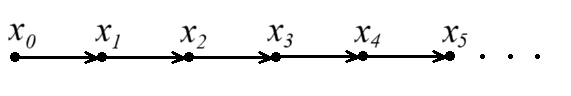
\includegraphics[width=0.5\textwidth]{free_unar_1}
		\caption{Свободный унар с единственным образующим $x_0$ (луч).}
	\end{figure}

	\begin{figure}
		\center
		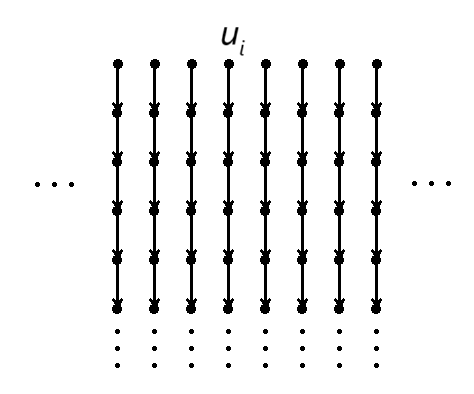
\includegraphics[width=0.4\textwidth]{free_unar_2}
		\caption{Свободный унар с множеством свободных образующих $\{ u_i \mid i \in I \}$.}
	\end{figure}
\end{frame}

\begin{frame}
	\frametitle{Унары}

	\begin{figure}
		\center
		
\includegraphics[width=0.45\textwidth]{line}
		\caption{Прямая (унар).}
	\end{figure}

	\begin{figure}
		\center
		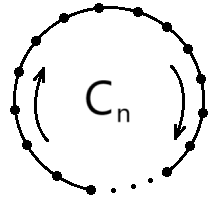
\includegraphics[width=0.15\textwidth]{cycle}
		\caption{Цикл $C_n$ длины $n$.}
	\end{figure}
\end{frame}

\begin{frame}
	\frametitle{Связные унары}

	\begin{definition}
		Унар $X$ называется \textit{связным}, если для любых $x_1, x_2 \in X$ существуют такие $i, j$, что $x_1 a^i = x_2 a^j$.
	\end{definition}

	\begin{figure}
		\center
		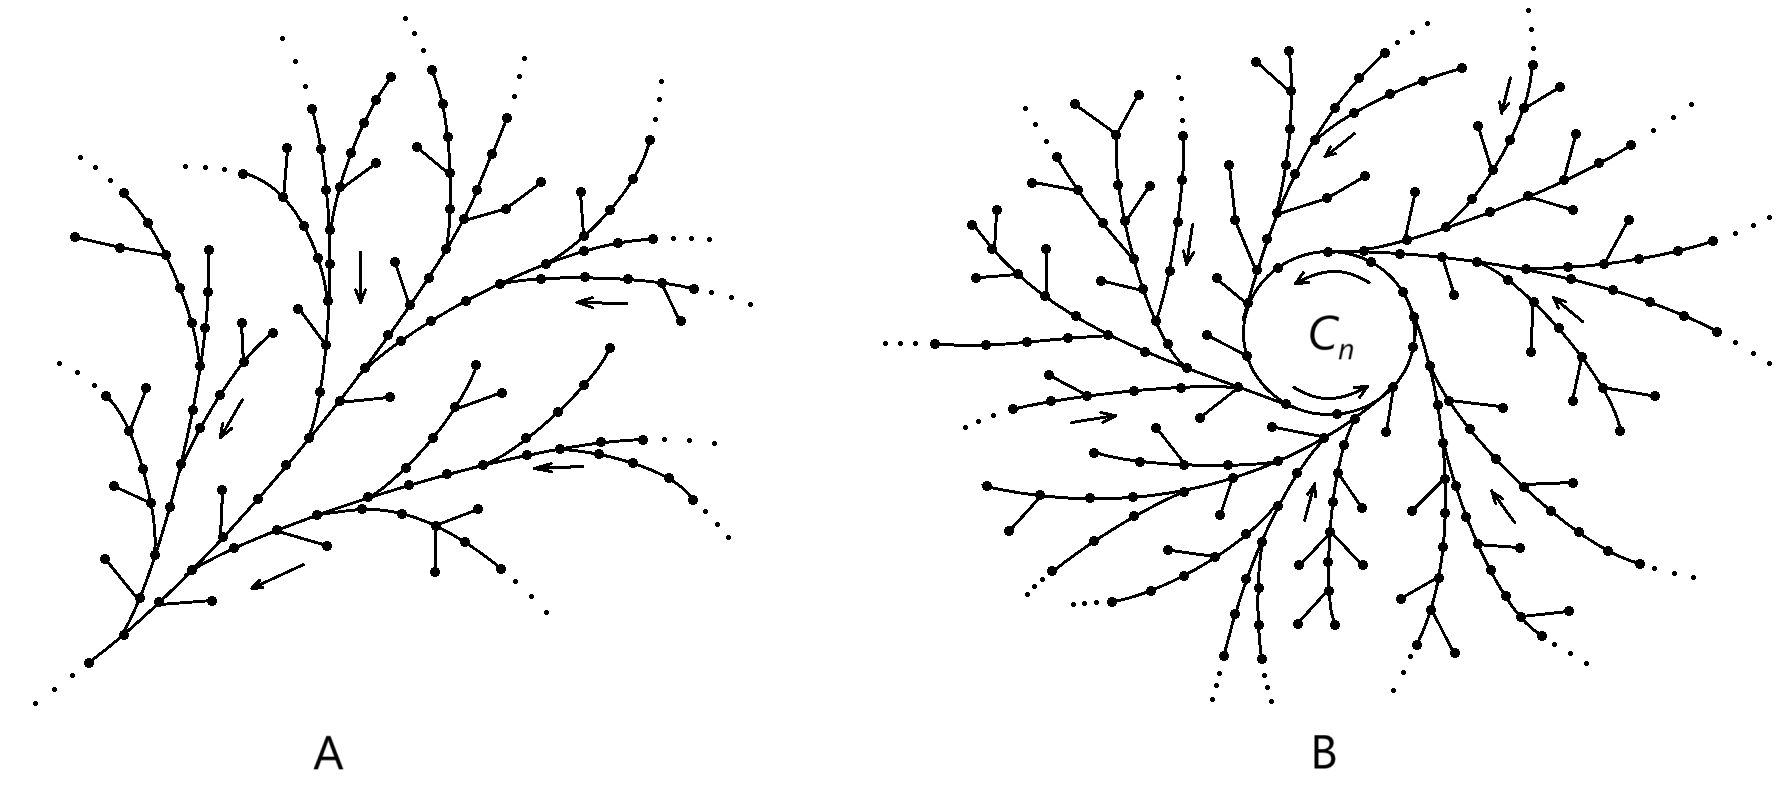
\includegraphics[width=1.0\textwidth]{connected_unars}
		\caption{Связные унары.}
	\end{figure}
\end{frame}

\begin{frame}
	\frametitle{Плоские унары}

	\begin{theorem}
		Унар $X$ является плоским в том и только том случае, если $X$ -- копроизведение унаров, являющихся прямыми, лучами или циклами\footcite[теорема]{flat_unars}.
	\end{theorem}
\end{frame}

\begin{frame}
	\frametitle{Полигоны, близкие к плоским}

	\begin{definition}
		Полигон $X$ называется\footcite[определения III.9.1 и III.8.1]{kilp}

		\begin{itemize}
			\item коуниверсально плоским, если функтор $X \otimes - $ сохраняет коуниверсальный квадрат;
			\item уравнительно плоским, если функтор $X \otimes - $ сохраняет уравнители;
			\item сильно плоским, если он является коуниверсально плоским и уравнительно плоским;
			\item плоским, если функтор $X \otimes - $ сохраняет мономорфизмы;
		\end{itemize}
	\end{definition}
\end{frame}

\begin{frame}
	\frametitle{Полигоны, близкие к плоским (продолжение)}

	\begin{definition}
		Полигон $X$ называется\footcite[определения III.9.1 и III.8.1]{kilp}

		\begin{itemize}
			\item слабо плоским, если функтор $X \otimes - $ сохраняет все вложения левых иделов в $S$;
			\item главно слабо плоским, если функтор $X \otimes - $ сохраняет все вложения главных левых идеалов в $S$;
			\item унаром без кручения, если $\forall x, x' \in X$, $\forall s \in S$ $xs = x's \rightarrow x = x'$.
		\end{itemize}

	\end{definition}
\end{frame}

\begin{frame}
	\frametitle{Условия (Р) и (Е)}

	\begin{definition}
		\begin{itemize}
			\item Будем говорить\footcite[определение III.9.4]{kilp}, что полигон $X$ над полугруппой $S$ удовлетворяет условию (P), если для него выполняется импликация: если $xs = x' s'$ для $x, x' \in X$, $s, s' \in S$, то существуют $x'' \in X$, $u,v \in S$ такие, что $x = x'' u$, $x' = x'' v$, $u s = v s'$;
			\item Полигон $X$ над полугруппой $S$ удовлетворяет условию (E), если для него выполняется импликация: если $x s = x s'$ для $x \in X$, $s, s' \in S$, то существуют $x' \in X$, $u \in S$ такие, что $x = x' u$, $us = us'$.
		\end{itemize}
	\end{definition}

\end{frame}

\begin{frame}
	\frametitle{Условия (Р) и (Е)}

	\begin{figure}
		\center
		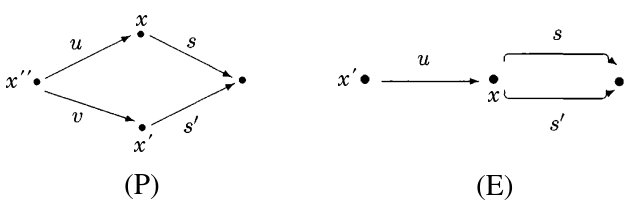
\includegraphics[width=0.8\textwidth]{p_and_e}
		\caption{Условия (Р) и (Е).}
	\end{figure}
\end{frame}

\begin{frame}
	\frametitle{Обзор}

	\begin{figure}
		\center
		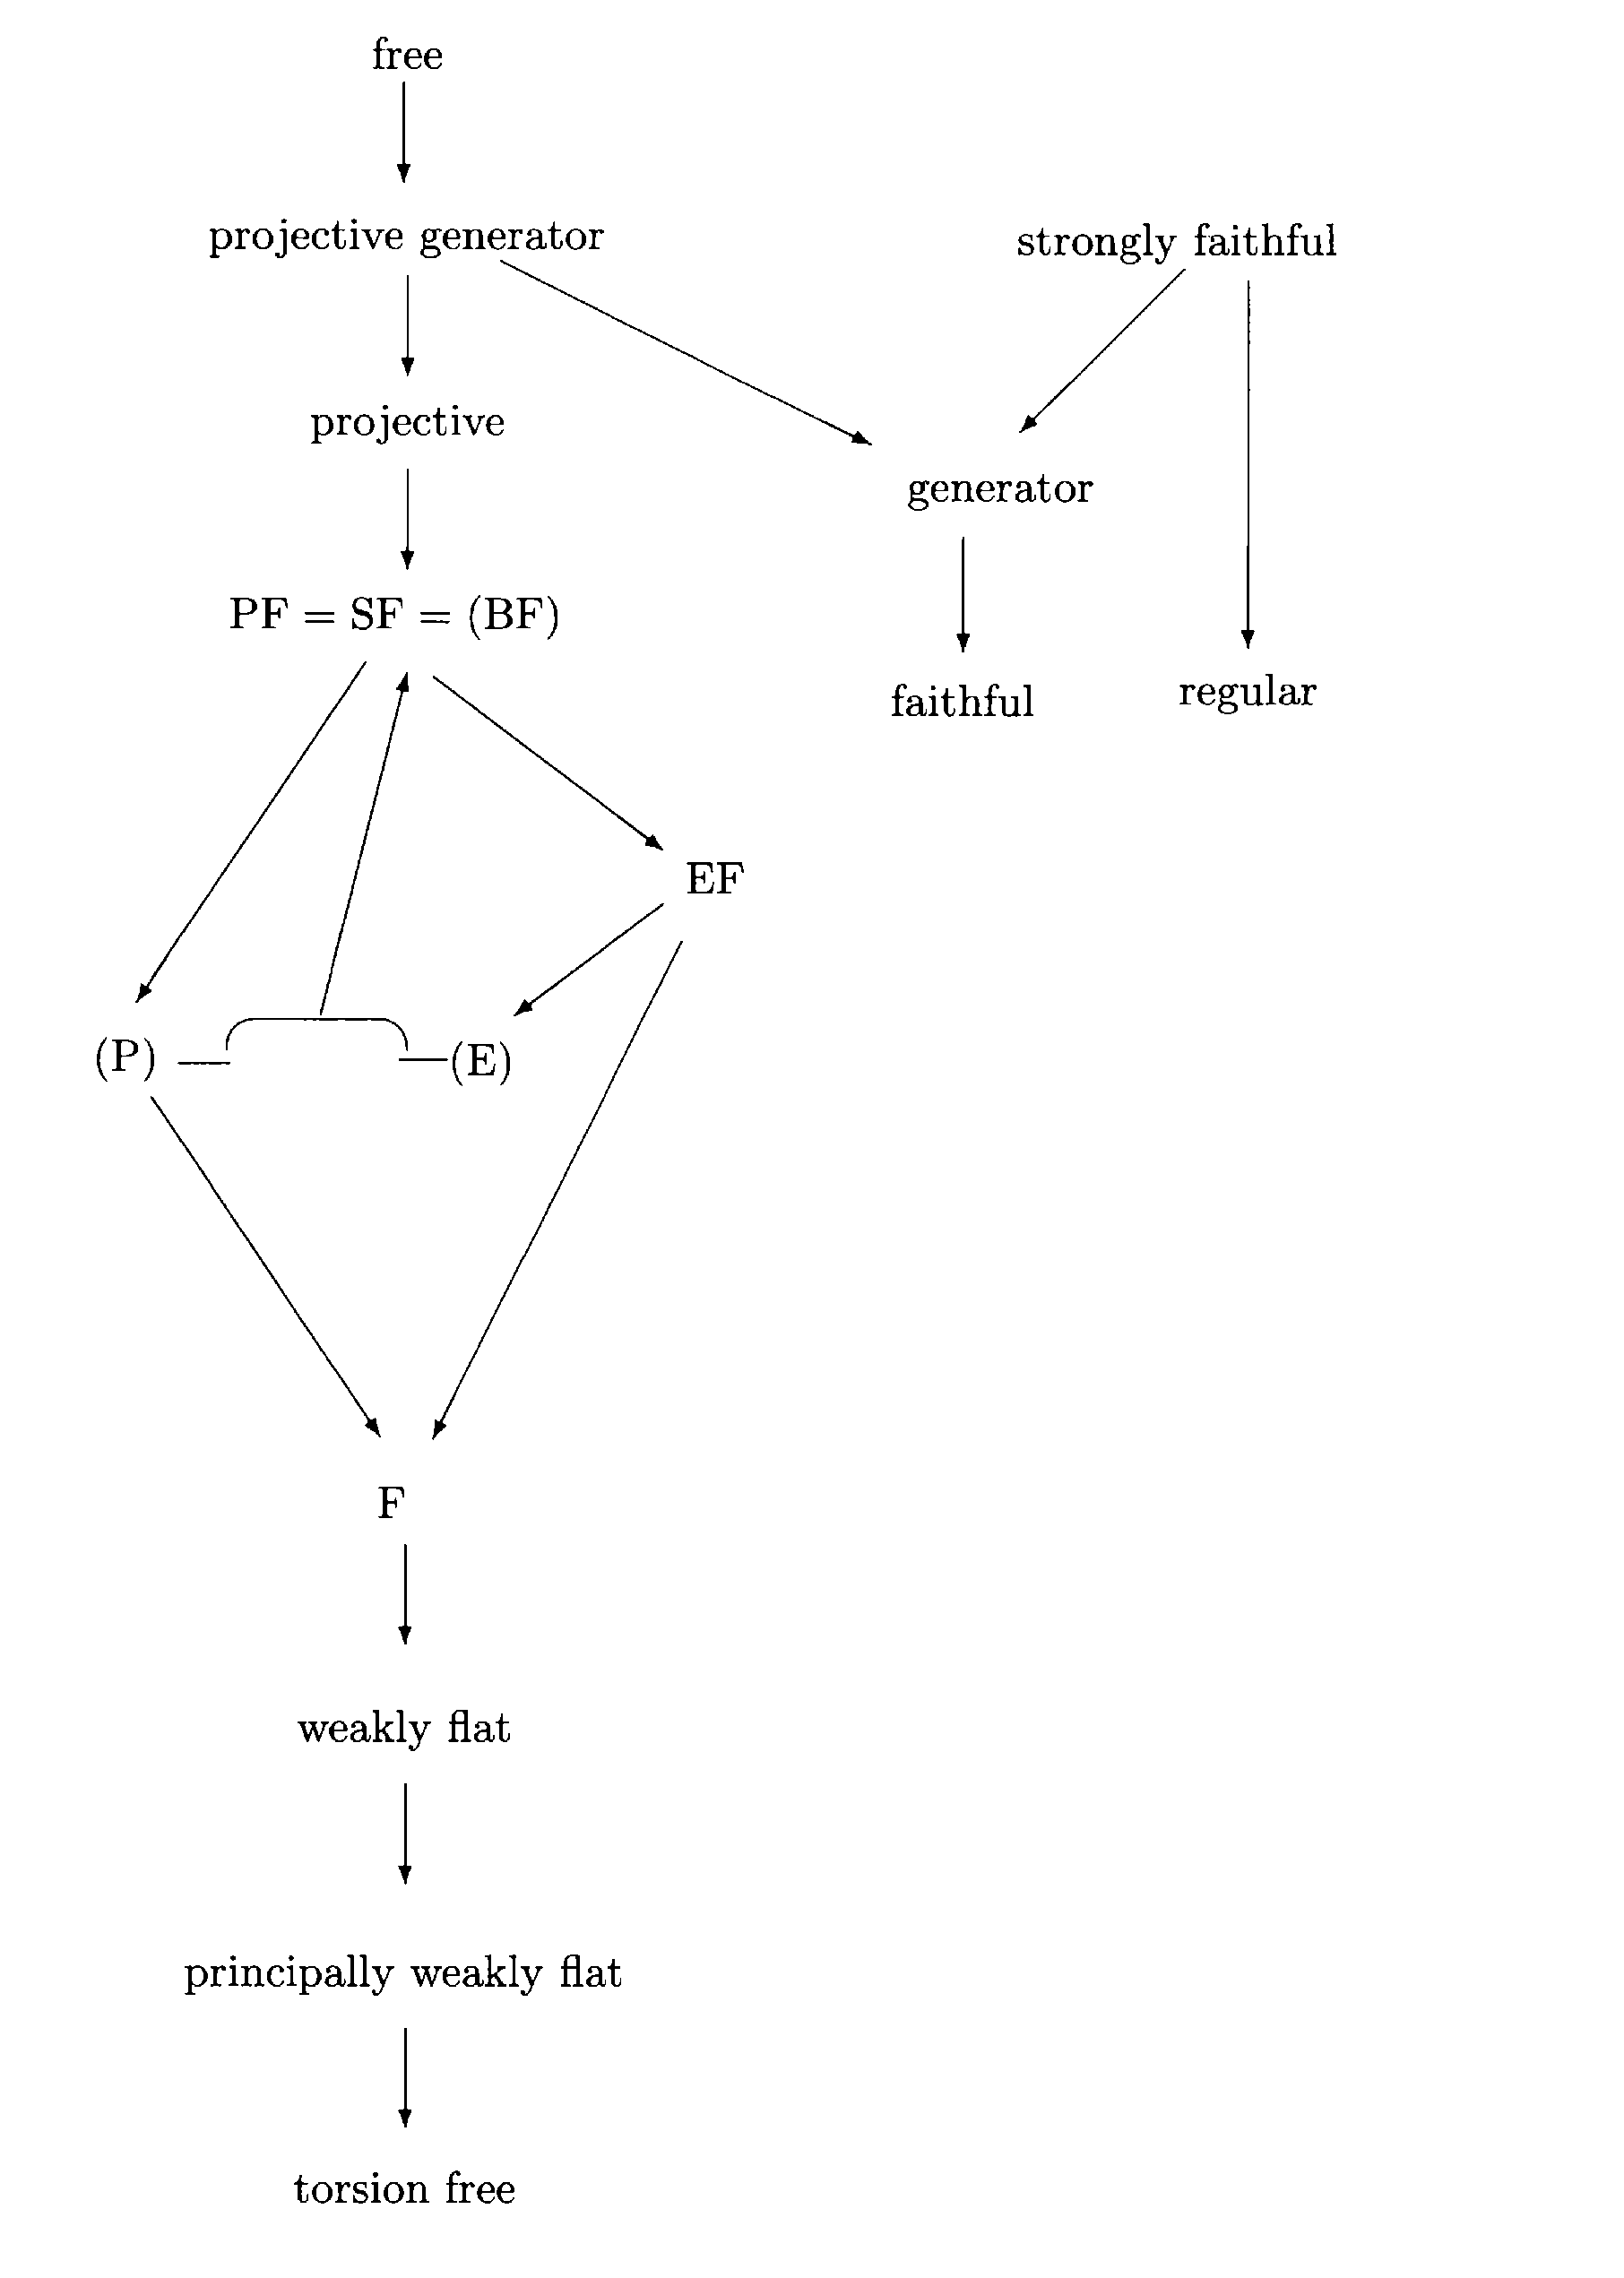
\includegraphics[width=0.5\textwidth]{overview_1.png}
	\end{figure}
\end{frame}

\begin{frame}
	\frametitle{Результаты}

	\begin{corollary}
		Для любого унара $X$ верны следующие эквивалентности:
		\begin{multline*}
			\text{(P)} \Leftrightarrow \text{плоский} \Leftrightarrow \text{слабо плоский} \Leftrightarrow \text{главно слабо плоский} \Leftrightarrow \\
			\Leftrightarrow \text{без кручения}.
		\end{multline*}
	\end{corollary}

	\begin{corollary}
		Для любого унара $X$ верны следующие импликации:
		\begin{gather*}
			\text{коуниверсально плоский} \Leftrightarrow \text{уравнительно плоский} \Rightarrow \text{(E)} \\
			\Leftrightarrow \text{строго точный} \Leftrightarrow \text{точный} \Leftrightarrow \text{регулярный.}
		\end{gather*}
	\end{corollary}
\end{frame}

\end{document}